\documentclass[11pt,letterpaper,oneside]{article}
\usepackage[top=0.5in,left=1.0in,right=1.0in,bottom=0.7in]{geometry}
%\usepackage[top=0.5in,left=1.8in,right=1.8in,bottom=1in]{geometry}
\usepackage{textcomp}
\usepackage{fancyvrb}
\usepackage{colortbl}
\usepackage[pdftex]{graphicx}
\DeclareGraphicsExtensions{.pdf}
\usepackage{caption}
\usepackage{subcaption}
\usepackage{url}
\usepackage{amsmath}
\usepackage[ruled,vlined,linesnumbered]{algorithm2e}

%\usepackage{setspace}
%\doublespacing

\title{Solving Graph Coloring Problem with SAT Solver}
\author{Dejun Qian}

\date{}

\begin{document}
\maketitle

\section{Introduction}
Many real world applications, like scheduling, register allocation and so on, can be modeled as graph coloring problem. It is important to find a solution to graph coloring problems efficiently. However, graph coloring problems are NP-hard, no polynomial time solutions have been found. Fortunately, graph coloring problem can be reduced to a well-studied NP-hard problem -- SAT problem \cite{reducibility}. People have designed a bunch of heuristic algorithms, and developed several SAT solvers to solve SAT problems.

This paper implements the algorithm to reduce a graph coloring problem to a SAT problem. The evaluation results show that the resulted algorithm can reduce a graph coloring problem to a SAT problem in polynomial time. We also implement our graph coloring solver using MiniSAT -- a light-weight and efficient SAT solver \cite{minisat}.

\section{Background}
\label{sec:background}
\subsection{Graph Coloring Problem}
A \textit{\textbf{k-coloring}} of an undirected graph $G=(V,E)$ is a function $c: V \rightarrow {1, 2, ..., k}$ such that $c(u) \neq c(v)$ for every edge $(u,v)$. In other words, the numbers $1,2,...,k$ represent the $k$ colors, and adjacent vertices must have different colors. The graph coloring problem asks the question about if there exists a \textit{k-coloring} of an undirected graph. If there is a \textit{k-coloring}, the solution should give an instance.

\subsection{SAT Problem and SAT solver}
A SAT problem asks about if there is some assignment of the values 0 and 1 to the variables of a boolean formula that causes the formula evaluates to 1. People usually write a boolean formula in \textit{\textbf{k-CNF}} (k-conjunctive normal form). We say a boolean formula is in \textit{k-CNF} if it is the AND of clauses of ORs of exactly k variables or their negations.

SAT problem is a NP-hard problem, no current methods can efficiently solve all SAT instances. However, researchers have developed a class of algorithms called SAT solvers that can efficiently solve a large enough subset of SAT instances. Examples of SAT solvers include: MiniSAT \cite{minisat}, Zchaff \cite{zchaff} and so on.

\section{Solving Graph Coloring Problem Using SAT solver}
\label{sec:implementation}
Both graph coloring problem and SAT problem are NP-hard problems, there are no existing polynomial solutions to them. These two problems can be reduced to each other in polynomial time \cite{reducibility}. As a lot of research has been done to develop SAT solvers that can solve a large set of SAT problems efficiently, we can transform the graph coloring problem to SAT problem first, use the SAT solver to solve the resulting SAT problem, and transform the solution of the SAT problem back to the solution of the original graph coloring problem.

\subsection{Graph Coloring to SAT}
The pseudocode that transforms a graph coloring problem to a SAT problem is shown in Algorithm \ref{alg:gc2sat}. The algorithms is composed of three parts: the first part enforces the two endpoints of each edge are colored with different colors; the second part enforces each vertex is colored; and the third part enforces each vertex is colored with no more than one colors. The time complexity for this algorithm is $O(k\cdot|E|+k^2\cdot|V|)$, we consider the operations for preparing the literals.

\begin{algorithm}[!h]
\DontPrintSemicolon
\SetKwComment{tcp}{\hfill$\triangleright$ }{}
\SetCommentSty{emph}
// enforce the edge constrains\;
\For{$\forall (v[i], v[j])\ in\ E$}{
  \For{$\forall$ c in 1..k}{
    emit clause ($\neg$ v[i,c] $\vee$ $\neg$ v[j,c])
  }
}
// ensure that every vertex is colored\;
\For{$\forall$ i in 1..$|V|$}{
  emit clause (v[i,1] $\vee$ v[i,2] $\vee$ .. $\vee$ v[i, k])
}
// ensure that every vertex is uniquely colored\;
\For{$\forall$ i in 1..$|V|$}{
  \For{$\forall$ c in 1..k}{
    \For{$\forall$ $c'$ in 1..k}{
      \If{$c \neq c'$}{
        emit clause ($\neg$ v[i,c] $\vee$ $\neg v[i,c']$)
      }
    }
  }
}
\caption{$\textsc{SAT-from-GC}(graph\ G=(V,E), limit\ k\ colors):$}
\label{alg:gc2sat}
\end{algorithm}

\subsection{SAT to Graph Coloring}
With the result of the corresponding SAT problem, we compute the result for the original graph coloring problem with Algorithm \ref{alg:sat2gc}. The algorithm receives the SAT assignment as input, find the atom whose value is 1, and determine the color for the related vertex.

\begin{algorithm}[!h]
\DontPrintSemicolon
\SetKwComment{tcp}{\hfill$\triangleright$ }{}
\SetCommentSty{emph}
// go through each assignment\;
a $\leftarrow$ [ ]\;
\If{v is empty} {
\Return a\;
}
\For{$\forall$ i in 1..$|V|$}{
  \For{$\forall$ c in 1..k}{
    \If{$v[i,c]$}{
      insert $(i,c)$ into a
    }
  }
}
\Return a\;
\caption{$\textsc{GC-from-SAT}(SAT\ assignment\ v, limit\ k\ colors):$}
\label{alg:sat2gc}
\end{algorithm}

\subsection{Solving SAT Problem with MiniSAT}
MiniSAT is a minimalistic, open-source SAT solver. It is released under MIT license, and is currently used on many projects. MiniSAT receives the SAT problem as a file in DIMACS CNF file format, writes the result in an output file. Our implementation generates the DIMACS CNF file, passes it to MiniSAT, and get the result from the output file of MiniSAT.

\subsection{Visualization}
We use dot \cite{dot} to visualize our graph coloring results. Figure \ref{fig:example} shows an example that illustrates a graph in figure \ref{fig:orig}, and the colored graph in figure \ref{fig:colored} with 3 colors.

\begin{figure}
  \centering
  \begin{subfigure}[b]{0.35\textwidth}
    \centering
    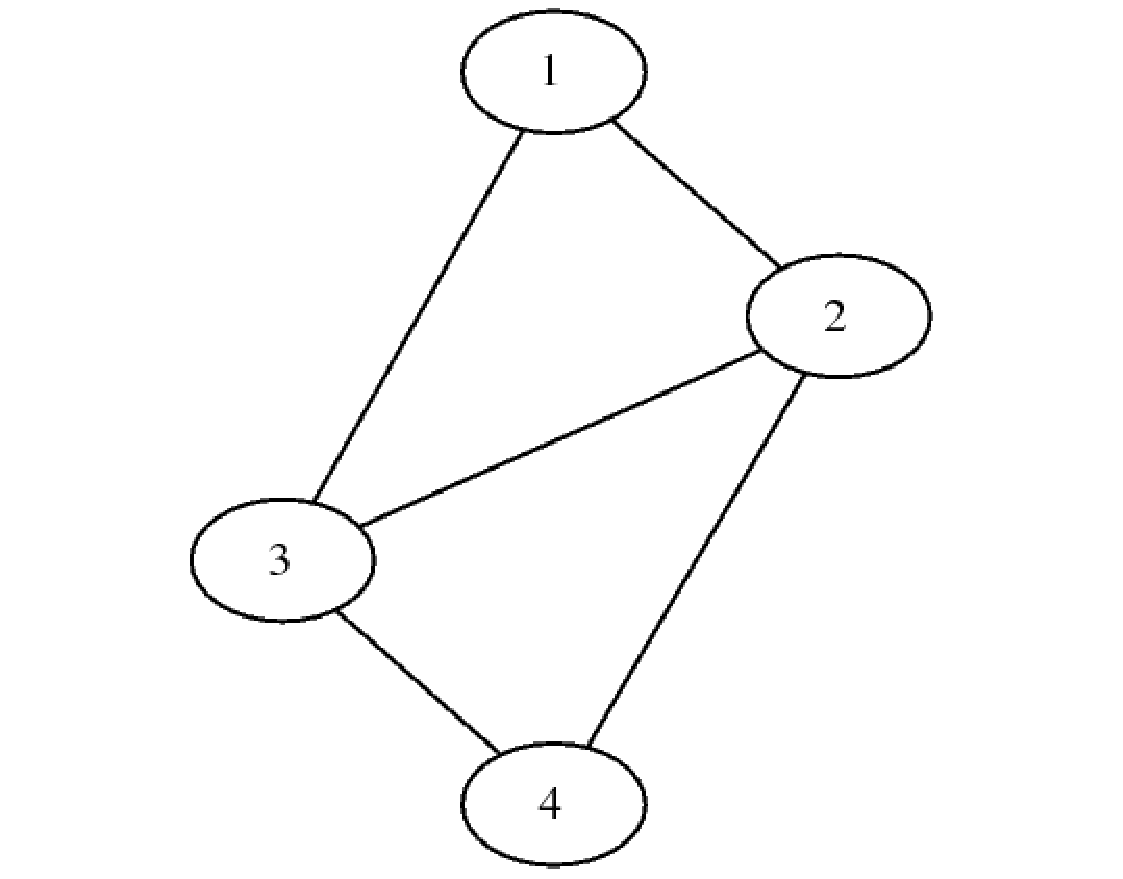
\includegraphics[width=\textwidth]{gc1}
    \caption{Original Graph}
    \label{fig:orig}
  \end{subfigure}%
  \begin{subfigure}[b]{0.35\textwidth}
    \centering
    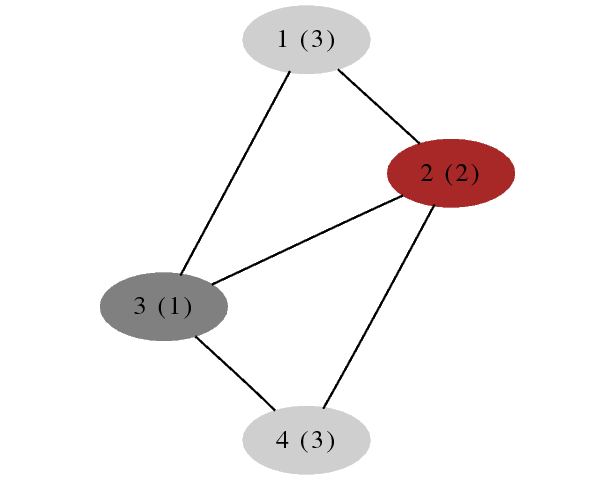
\includegraphics[width=\textwidth]{gc2}
    \caption{Colored Graph}
    \label{fig:colored}
  \end{subfigure}
  \caption{An example graph and its colored graph}\label{fig:example}
\end{figure}

\section{Evaluation}
\label{sec:evaluation}
Figure \ref{fig:evaluation} shows the running time of the algorithm. Figure \ref{fig:vertex} and \ref{fig:edge} shows the running time goes linearly when the number of vertex and edge changes. Figure \ref{fig:color} shows the running time goes quadratically when the number of colors changes. The results match the analytical result $O(k\cdot|E|+k^2\cdot|V|)$.

\begin{figure}
  \centering
  \begin{subfigure}[b]{0.3\textwidth}
    \centering
    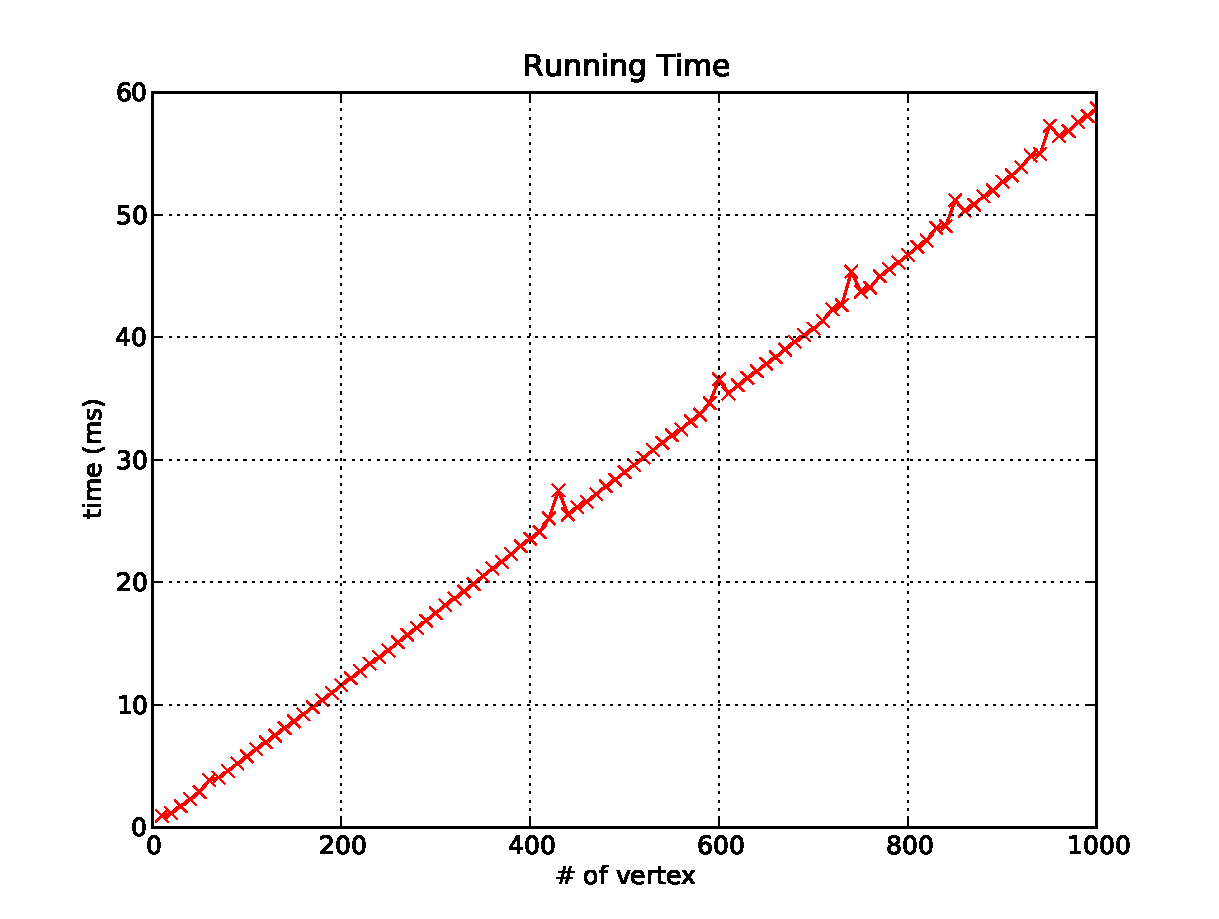
\includegraphics[width=\textwidth]{fig1}
    \caption{Different \# of vertex}
    \label{fig:vertex}
  \end{subfigure}%
  \begin{subfigure}[b]{0.3\textwidth}
    \centering
    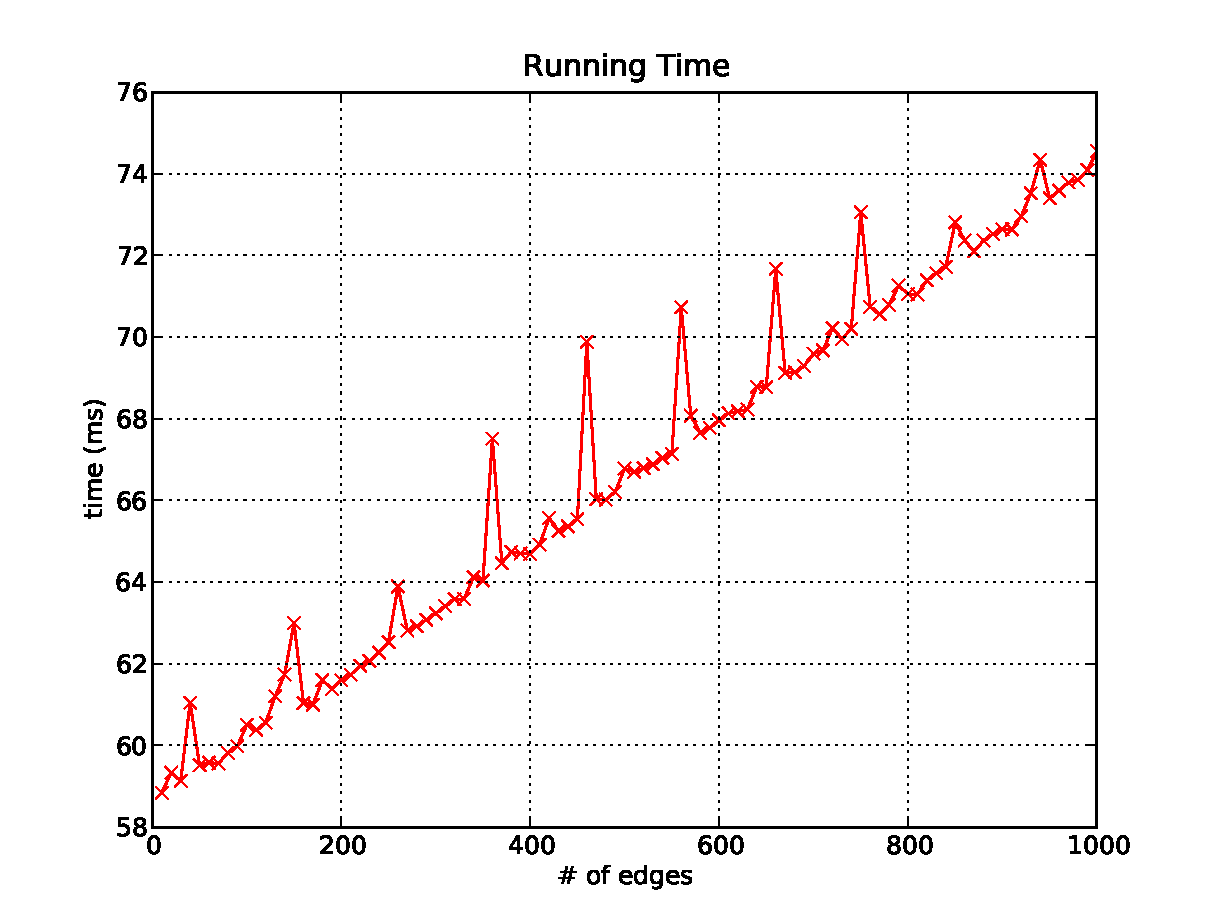
\includegraphics[width=\textwidth]{fig2}
    \caption{Different \# of edges}
    \label{fig:edge}
  \end{subfigure}%
  \begin{subfigure}[b]{0.3\textwidth}
    \centering
    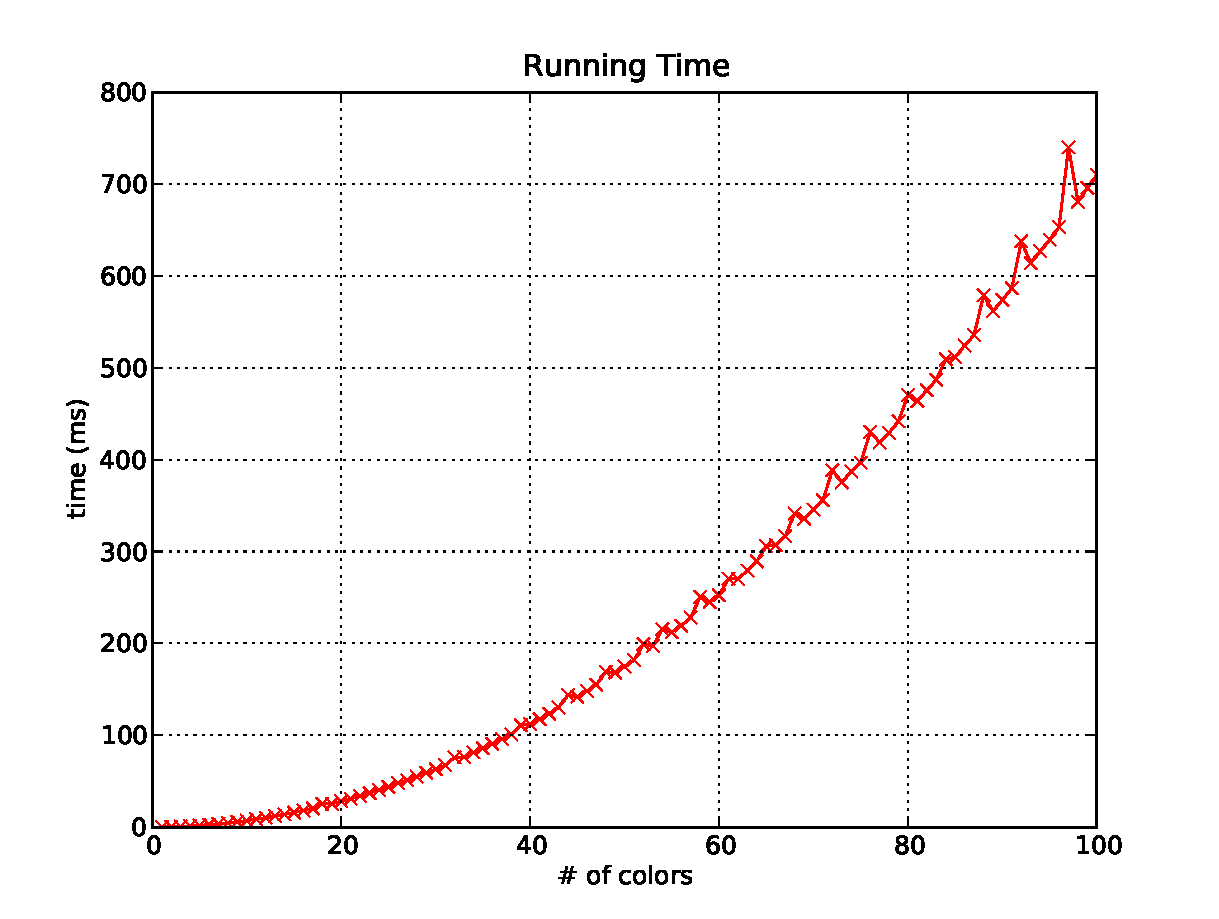
\includegraphics[width=\textwidth]{fig3}
    \caption{Different \# of colors}
    \label{fig:color}
  \end{subfigure}
  \caption{Running time for the algorithm}\label{fig:evaluation}
\end{figure}


\section{Conclusion}
\label{sec:conclusion}
This paper implements the algorithm that can reduce graph coloring problem to a SAT problem. The evaluation results show that the algorithm runs in polynomial time in terms of the number of vertexes, the number of edges and the number of colors.

\bibliographystyle{acm}
\bibliography{reference}

\end{document}
